\documentclass[../main.tex]{subfiles}

\graphicspath{{../images/}}

\begin{document}
\hrule
\section{Bound States}
\hrule \vspace{10px}

\lhead{Lecture 10: 2/19/24}
\chead{Bound States}
\rhead{PHYS 474}

\paragraph*{Two Types:}
\begin{itemize}
    \item Binding Energy $<$ Rest mass energy: Nonrelativistic bound state e.g. Hydrogen atom
    (-13.6 eV $<$ 1GeV rest mass of proton). 
    \item Binding Energy $>$ Rest mass energy: Relativistic bound state e.g. light meson.
\end{itemize}
\paragraph*{Hydrogen Atom:} The potential energy is given by
\begin{align*}
    V(r) = -\frac{e^2}{r}
\end{align*}
or the coulomb potential. The Hamiltonian is given by the Schr\"odinger equation
\begin{align*}
    H\psi = -\frac{\hbar}{2m} \laplacian \psi(\vb r) + V(r) \psi(\vb r) = E\psi(\vb r)
\end{align*}
where $V(r)$ is the central potential with spherical symmetry SO(3). But there also is an enhanced 
symmetry.
\paragraph*{Noether's Theorem:} Symmetry $\leftrightarrow$ Conservation Law. e.g. 
\begin{itemize}
    \item SO(3) $\leftrightarrow$ Conservation of Angular momentum. 
    \item SO(1,3) $\leftrightarrow$ linear momentum (Poincare symmetry)
    \item T-reversal $\leftrightarrow$ energy
    \item U(1)$_{em}$ $\leftrightarrow$ electric charge
\end{itemize}
so from the central potential, we know that angular momentum $\vb L$ is conserved. But for
$1/r$ there is a SO(4) symmetry from the LRL (Laplace-Runge-Lenz) vector
\begin{align*}
    \mathcal{L} = \frac{1}{m} \vb L \cross \vb p + \frac{\kappa \vb r}{r}
\end{align*}
where
\begin{align*}
    V(r) = -\frac{\kappa}{r}
\end{align*}
the energy eigenvalues of the hydrogen atom are given by
\begin{align*}
    E_n = -\frac{\qty{13.6}{eV}}{n^2} = -\frac{m e^4}{2\hbar^2 n^2}
     = -\frac{1}{2} \frac{\alpha m_e c^2}{n^2}
\end{align*}
where $\alpha = \frac{e^2}{\hbar c} \approx \frac{1}{137}$ is the fine structure constant.
\paragraph*{Degeneracy} $n^2$ e.g.
% table of n l m and degeneracy
\begin{table}[ht]
    \centering
    \begin{tabular}{c|c|c|c}
        n & l & m & degeneracy \\
        \hline
        1 & 0 & 0 & 1 \\
        \hline
        2 & 0 & 0 & 1 \\
         & 1 & -1,0,1 & 3 \\
        \hline
        3 & 0 & 0 & 1 \\
        & 1 & -1,0,1 & 3 \\
        & 2 & -2,-1,0,1,2 & 5 \\
    \end{tabular}
\end{table}
For SO(3), $(2l + 1)$ degeneracy
\begin{align*}
    \sum_{l=0}^{n-1} (2l + 1) = 2\sum_{l=0}^{n-1} l + n = 2 \frac{(n - 1)(n)}{2} + n = n^2
\end{align*}
\paragraph*{Positronium} ($e^+ e^-$ bound state) has the same energy levels as the hydrogen atom
the energy eigen value is given by first looking at the reduced mass
\begin{align*}
    \mu = \frac{1}{\frac{1}{m_e} + \frac{1}{m_e}} = \frac{m_1m_2}{m_1 + m_2} \approx m_1    
    \qqtext{if} m_1 \ll m_2
\end{align*}
but here $m_1 = m_2 = m_e$ so $\mu = \frac{m_e}{2}$. The energy eigenvalues are given by
\begin{align*}
    E_n = \frac{1}{2} -\frac{\qty{13.6}{eV}}{n^2} = -\frac{\qty{6.8}{eV}}{n^2}
\end{align*}
We can do this for Muonium ($\mu^+ e^-$ bound state) and Pionic Hydrogen($\pi^+ e^-$ bound state).
\paragraph*{Fine Structure}
\begin{enumerate}
    \item Relativistic Correction
    \begin{align*}
        T = E - m_ec^2
    \end{align*}
    \item Spin-Orbit Coupling
    \item Lambd Shift (QED)
    \item Hyperfine Splitting aka zeeman effect
\end{enumerate}

\newpage
\lhead{Lecture 11: 2/21/24}

\paragraph*{Quiz Review} 
\begin{itemize}
    \item For the Positronium:
    \begin{align*}
        C: (-1)^{l+s} = (-1)^n
    \end{align*}
    where $l + s = n$ (the selection rule for Positronium decay). *for $n$ photons, $C = (-1)^n$. 
    FOr the ground states $l = 0$ so the spin is
    \begin{align*}
        S: \ohf \otimes \ohf = 1 \oplus 0
    \end{align*}
    where we have a triplet state $S = 1$ and a singlet state $S = 0$. For this singlet:
    \begin{align*}
        S = 0 \implies (-1)^0 = 1 = (-1)^2
    \end{align*}
    or two photons can be emitted (para-positronium). For the triplet state:
    \begin{align*}
        S = 1 \implies (-1)^1 = -1 = (-1)^3
    \end{align*}
    or three photons can be emitted (ortho-positronium). The mass of each photon for two photons is
    roughtly a half of the mass of the positronium $E_\gamma = \qty{511}{keV}$. For three photons
    $E_\gamma < 511$ keV. 
    \item Binding Energy vs. Rest Mass Energy: Quarkonium ($q \bar q$): $uds$ light quarks,
    $cbt$ heavy quarks.
    \begin{itemize}
        \item Heavy Quarkonium: $c\bar c$: Charmonium ($J/\psi$), $b\bar b$: Bottomonium
        ($\Upsilon$), $t\bar t$: Toponium \emph{does not exist}
        (very heavy so it decays really fast $\sim 10^{-25}$s vs
        $\tau_{\text{bound state}} \sim 10^{-23}$ sec).
    \end{itemize}
    For Charmoniun, the reduced mass is 
    \begin{align*}
        \mu = \frac{m_c m_c}{m_c + m_c} \approx \frac{m_c}{2}
    \end{align*}
    and the energy of the Hydrogen atom is
    \begin{align*}
        E_n = -\frac{m e^4}{2\hbar^2 n^2} = -\frac{1}{2} \frac{\alpha m c^2}{n^2}
    \end{align*}
    and for the Charmonium:
    \begin{align*}
        E_n = -\frac{4}{9} \frac{1}{2} \frac{\alpha m_c c^2}{n^2} \qqtext{incorrect}
    \end{align*}
    where we have to adjust for the charge of the quark $e \to \frac{2}{3}e$ and the potential:
    For electron coulomb potential we know that 
    \begin{align*}
        V = -\frac{e^2}{r} = -\frac{e^2}{\hbar r}\frac{\hbar c}{r} = -\frac{\alpha \hbar c}{r}
    \end{align*}
    but for quarks there is a different potential from the strong interaction (gluon)
    \begin{align*}
        V(r) = -\frac{\alpha_s \hbar c}{r} - \frac{4}{9} \frac{\alpha \hbar c}{r}
        \qquad \alpha_s = \frac{g_s^2}{\hbar c} \gg \alpha
    \end{align*}
    which is much larger than the coulomb potential (suppressed second term), but there is a
    transition to a linear potential as the distance get very large.
    \begin{align*}
        V(r) = -\frac{4}{3} \frac{\alpha_s \hbar c}{r} + F_o r \qqtext{QCD Potential}
    \end{align*}
    there also is a color factor $\frac{4}{3}$ based on the three colors of the quarks.
    So the energy is given by
    \begin{align*}
        E_n = -\frac{4}{3} \frac{1}{2} \frac{\alpha_s m_c c^2}{n^2}
    \end{align*}
    \item Decay of Charmonium:
    \begin{align*}
        J/\psi \to \pi^+ \pi^- \pi^0 \qor D^+ D^-
    \end{align*}
    For the ground state, $m_{J/\psi} = 3.1$ GeV. And the total rest mass of $D^+ D^-$ is 
    kinematically forbidden $m_{D^+} + m_{D^-} = 3.7$ GeV. We have a decay to 3 pions due to
    the G-parity conservation $(-1)^I C$ or $(-1)^{n}$.

    \paragraph*{OZI rule} (Okubo, Zweig, Iizuka) Cutting a hard gluon line in the Feynman diagram
    separates the quarks and the decay is suppressed. For soft gluon lines, cutting a line does not
    separate the quarks and the decay is not suppressed.
    \begin{figure}[ht]
        \centering
        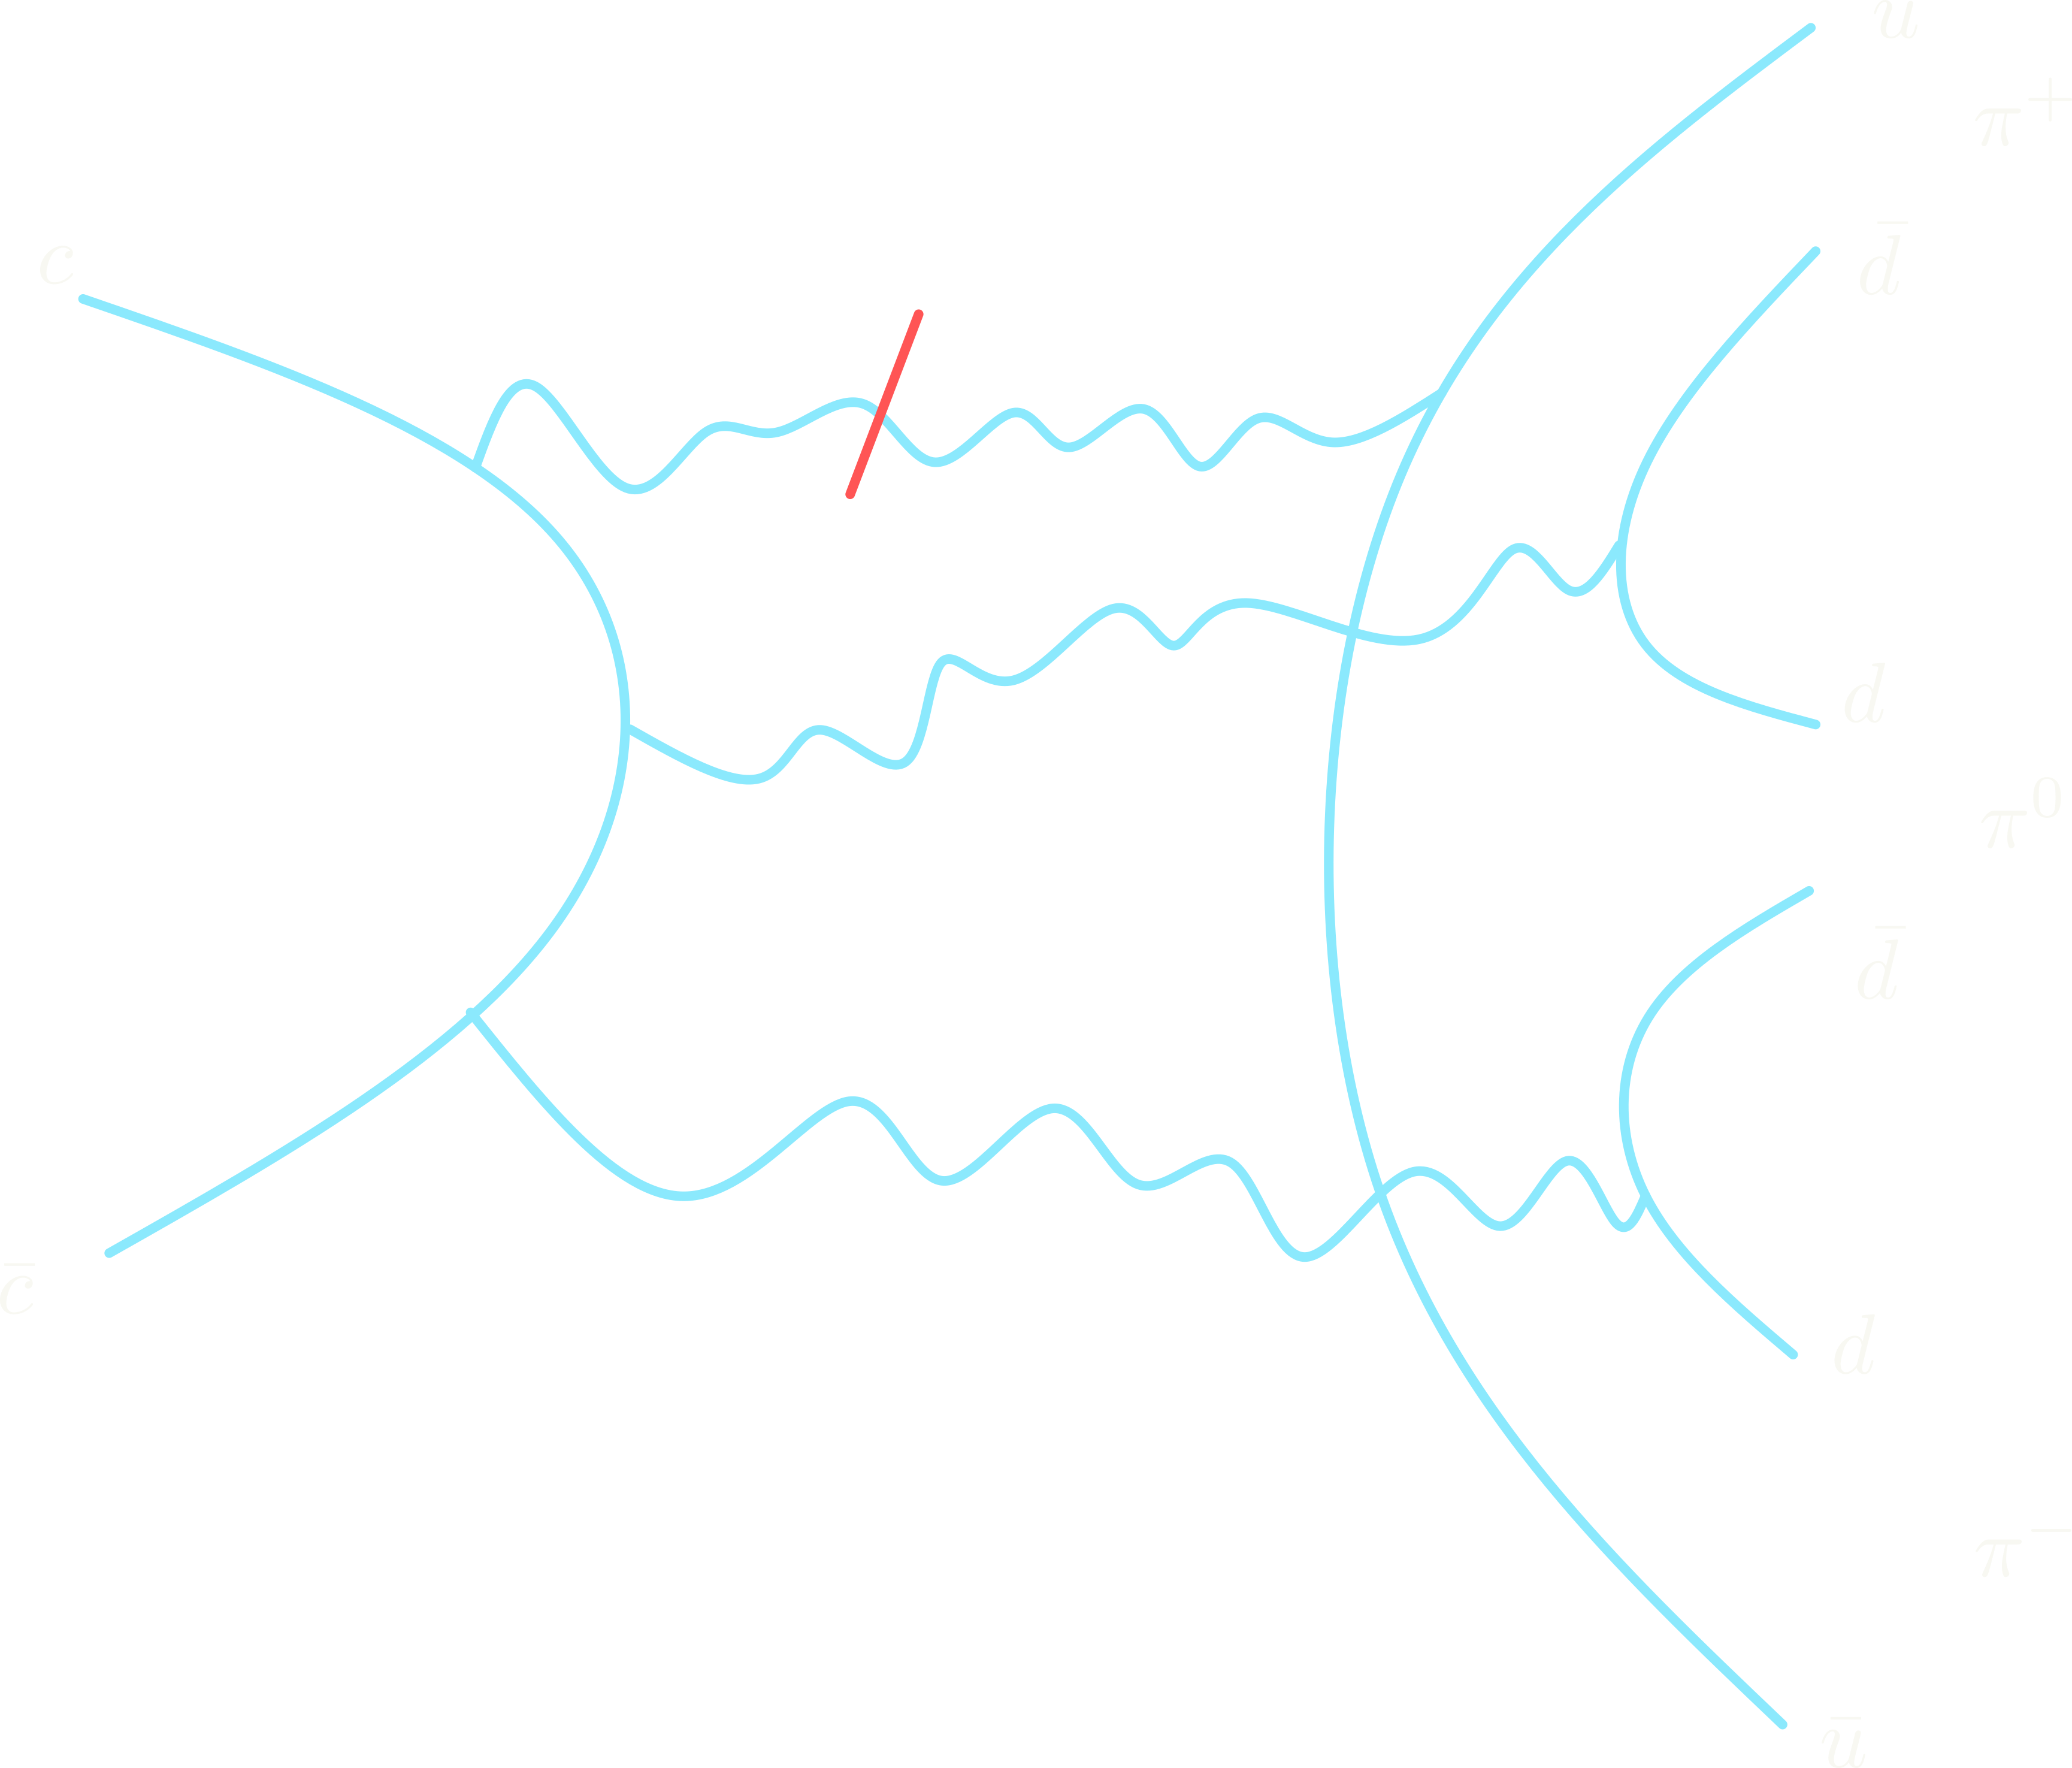
\includegraphics[width=0.5\textwidth]{ozirule.png}
        \caption{OZI Rule}
        \label{fig:ozi}
    \end{figure}
    \item Light Mesons: $q\bar q$ where $q = u,d,s$. There are nine spin-0 (pseudo scalar) mesons
    and nine spin-1 (vector) mesons. (insert figure 5.11 from Griffiths). From the lie algebra
    of the spin-0 nonet
    \begin{align*}
        3 \otimes \bar 3 = 8 \oplus 1
    \end{align*}
    where the 1 is the $\eta'$ meson. and we break down the 8 into
    \begin{align*}
        8 \to 2 \oplus 3 \oplus 2 \oplus 1
    \end{align*}
    where they refer to the top row, middle row pions, bottom row and $\eta$ meson. For the vector
    mesons. For the isospin doublet:
    \begin{align*}
        u = \ket{\ohf \ohf} \qquad d = \ket{\ohf -\ohf}
    \end{align*}
    and for the antiquarks:
    \begin{align*}
        \bar u = \ket{\ohf -\ohf} \qquad \bar d = -\ket{\ohf \ohf}
    \end{align*}
    and the pions are given by
    \begin{align*}
        \pi^+ &= \ket{\ohf \ohf} \otimes \ket{\ohf \ohf} = - u \bar d \\
        \pi^- &= \ket{\ohf -\ohf} \otimes \ket{\ohf -\ohf} = d \bar u \\
        \pi^0 &= \frac{1}{\sqrt{2}}
            \qt(\ket{\ohf -\ohf} \otimes \ket{\ohf \ohf} + \ket{\ohf \ohf} \otimes \ket{\ohf -\ohf})  \\
        &= \frac{1}{\sqrt{2}} (u \bar u - d \bar d)
    \end{align*}
    for the corner mesons:
    \begin{align*}
        K^0 = d \bar s \qquad \bar K^0 = \bar d s \qquad K^+ = u \bar s \qquad K^- = \bar u s
    \end{align*}
    and the $\eta$ mesons are
    \begin{align*}
        \eta' &= \frac{1}{\sqrt{3}} (u \bar u + d \bar d + s \bar s) \\
        \eta &= \frac{1}{\sqrt{6}} (u \bar u + d \bar d - 2s \bar s)
    \end{align*}
    For spin-1 mesons, in terms of the flavor
    \begin{align*}
        \rho^+, \rho^0, \rho^- = \pi^+, \pi^0, \pi^- 
    \end{align*}
    and the same for the $K^*$ mesons. The difference is in the center
    \begin{align*}
        \omega = \frac{1}{\sqrt{2}} (u \bar u + d \bar d) \qquad \phi = s \bar s
    \end{align*}
\end{itemize}

\newpage
\lhead{Lecture 12: 2/26/24}
\paragraph*{Quiz Review:}
For the kinetic energy of a particle
\begin{align*}
    T &= E - mc^2 \\
    &= \sqrt{\abs{\vb p}^2c^2 + m^2c^4} - mc^2 \\
    &= mc^2\qt(1 + \frac{\vb p^2}{m^2c^2})^{1/2} - mc^2 \\
\end{align*}
and using the binomial expansion
\begin{align*}
    (1 + x)^n \approx 1 + nx + \frac{1}{2} \frac{n(n-1)}{2} x^2 \dots \qqtext{for} x \ll 1
\end{align*}
so
\begin{align*}
    T &= mc^2 \qt(\cancel 1 + \frac{\vb p^2}{2m^2c^2} - \frac{\vb p^4}{8m^4c^4} + \dots) - \cancel {mc^2} \\
    &= \frac{\vb p^2}{2m} - \frac{1}{8} \frac{\vb p^4}{m^3c^2} + \dots
\end{align*}
From last time: Light mesons $(u, d, s)$ with $q\bar q$ bound states and spin
\begin{align*}
    \ohf \otimes \ohf = 1 \oplus 0
\end{align*}
where we for the spin-0 pseudoscalar mesons: $\pi, K, \eta$ we have 9 states. And for the spin-1
vector mesons: $\rho, K^*, \omega, \phi$ we have 9 states. The flavor states of $K$ mesons:
\begin{align*}
    K^+: (u\bar s) \quad K^-:(\bar u s) \quad K^0: (d\bar s) \quad \bar K^0: (\bar d s)
\end{align*}
and for vector $K$ mesons
\begin{align*}
    K^{*+}: (u \bar s) \qqtext{etc.}
\end{align*}
so the Isospin states
\begin{align*}
    \mqty(u \\ d) \otimes \mqty(\bar d \\ \bar u) = 1 \oplus 0
\end{align*}
so 
\begin{itemize}
    \item spin-0: $1\sim \pi^+, \pi^-, \pi^0$, $0 \sim \eta$
    \item spin-1: $1 \sim \rho^+, \rho^0, \rho^-$, $0 \sim \omega$
\end{itemize}
and in $SU(3)$: 
\begin{align*}
    3 \otimes \bar 3 = 8 \oplus 1
\end{align*}
where $\eta'$ is the spin-0 singlet (1). We can break down the spin algebra to isospin
\begin{align*}
    \mqty(\uparrow \\ \downarrow) \otimes \mqty(\uparrow \\ \downarrow)
        = \mqty(u \\ d) \otimes \mqty(\bar d \\ \bar u) = 1 \oplus 0
\end{align*}
where
\newcommand{\ua}{\uparrow}
\newcommand{\da}{\downarrow}
\begin{align*}
    \ket{1,1} &= \ket{\ua \ua} \\
    \ket{1,0} &= \frac{1}{\sqrt{2}} (\ket{\ua \da} + \ket{\da \ua}) \\
    \ket{1,-1} &= \ket{\da \da} \\
    \ket{0,0} &= \frac{1}{\sqrt{2}} (\ket{\ua \da} - \ket{\da \ua})
\end{align*}
and the charge conjugation operator
\begin{align*}
    C u \to \bar u \qquad C d \to \bar d \\
    C = i \sigma^2 = i \mqty(0 & -i \\ i & 0) = \mqty(0 & 1 \\ -1 & 0) \\
    C\mqty(u \\ d) \to \mqty(-\bar d \\ \bar u)
\end{align*}
so
\begin{align*}
    \ket{1,1} = -u \bar d = \ket{\pi^+}, \ket{\rho^+} \\
    \ket{1,0} = \frac{1}{\sqrt{2}} (u \bar u - d \bar d) = \ket{\pi^0}, \ket{\rho^0} \\
    \ket{1,-1} = \bar u  d = \ket{\pi^-}, \ket{\rho^-} \\
    \ket{0,0} = \frac{1}{\sqrt{2}} (u \bar u + d \bar d) = \cancel{\ket{\eta}}, \ket{\omega}
\end{align*}
where the $\eta$ is not correct. We know that $\psi$ is orthgonal to $\omega$ so
\begin{align*}
    \ket{\psi} = \ket{s \bar s}
\end{align*}
we know that $\eta'$ is an $SU(3)$ singlet so
\begin{align*}
    \ket{\eta'} = \frac{1}{\sqrt{3}} (u \bar u + d \bar d + s \bar s)
\end{align*}
and since $\eta$ is orthogonal to $\eta'$ and all other states:
\begin{align*}
    \ket{\eta} = \frac{1}{\sqrt{6}} (u \bar u + d \bar d - 2s \bar s)
\end{align*}
this is a special case for the pseudoscalar light mesons. Even though the spin-0 and spin-1
particles are made of the same quarks, their masses are very different! So the true meson mass is
\begin{align*}
    M = m_1 + m_2 + A \frac{\vb S_1 \cdot \vb S_2}{m_1 m_2}
\end{align*}
this third term is the spin-spin interaction from the Hydrogen Atom ($n^2$ degeneracry) 
hyperfine splitting. The spin-spin interaction breaks the degeneracy of the $n^2$ states. Finding
\begin{align*}
    \vb S_T &= \vb S_1 + \vb S_2 \\
    \vb S^2 &= (\vb S_1 + \vb S_2)^2 \\
    &= \vb S_1^2 + \vb S_2^2 + 2\vb S_1 \cdot \vb S_2
\end{align*}
Where from the operator
\begin{align*}
    [J^2, J_z] = 0 \qquad \ket{j, m} \\
    J_z \ket{j,m} + \hbar m \ket{j,m} \\
    J^2 \ket{j,m} = \hbar^2 j(j+1) \ket{j,m}
\end{align*}
so the eigenvalues of $\vb S$ are $\ohf(\ohf + 1)\hbar^2$:
\begin{align*}
    \vb S^2 &= \thf \hbar^2 + \thf \hbar^2 + 2\vb S_1 \cdot \vb S_2 \\
    &= \frac{3}{2}\hbar^2 + 2\vb S_1 \cdot \vb S_2
\end{align*}
so for the scalar case $s =0$, $\vb S^2 = 0$:
\begin{align*}
    \vb S_1 \cdot \vb S_2 = -\frac{3}{4}\hbar^2
\end{align*}
and for the vector case $s = 1$, $\vb S^2 = 2\hbar^2$:
\begin{align*}
    \vb S_1 \cdot \vb S_2 = \ohf \qt(2 - \thf \hbar^2)
\end{align*}
So
\begin{align*}
    \vb S_1 \cdot \vb S_2 = \begin{cases}
        -\frac{3}{4}\hbar^2 & \text{spin-0} \\
        \frac{1}{4} \hbar^2 & \text{spin-1}
    \end{cases}
\end{align*}
e.g. we have meson masses
\begin{itemize}
    \item $(u,d): m_\rho = \qty{775}{MeV/c^2}$
    \item $(u,d): m_\pi = \qty{140}{MeV/c^2}$
\end{itemize}
And we have an effective mass (MIT bag model):
\begin{align*}
    m_{eff} \geq \Lambda_{QCD} \sim \qty{200}{MeV/c^2}
\end{align*}
Quarks are always in bound states, and do not feel the strong interaction. And the bare mass is 
different from the effective mass. Some bare masses:
\begin{align*}
    m_{u,d} \sim \qty{300}{MeV/c^2} \\
    m_s \sim \qty{400}{MeV/c^2}
\end{align*}
\paragraph*{Baryons\dots} (light): $qqq$ bound states. We can treat the 3 body system as a 2 body
system(CM of 2 quarks plus the third quark). For the ground state, $l = l' = 0$ for simplicity.
\paragraph*{Spin configurations}
\begin{align*}
    \ohf \otimes \ohf \otimes \ohf &= (1 \oplus 0) \otimes \ohf \\
    &= (1 \otimes \ohf) \oplus (0 \otimes \ohf) \\
    &= (\thf \oplus \ohf) \oplus (\ohf) \\
    &= 4 \oplus 2 \oplus 2
\end{align*}
(the 3/2 spin has 4 states: $3/2, 1/2, -1/2, -3/2$) where
\begin{align*}
    j_1 \otimes j_2 = (j_1 + j_2), \dots, \abs{j_1 - j_2}
\end{align*}
we also have 8 spin states for the 3 quarks:
\begin{align*}
    \ua \ua \ua \\
    \ua \ua \da, \ua \da \ua, \da \ua \ua \\
    \ua \da \da, \da \ua \da, \da \da \ua \\
    \da \da \da
\end{align*}
so
\begin{align*}
    \ket{\thf,\thf} &= \ket{\ua\ua\ua} \\
    \ket{\thf,\ohf} &= \frac{1}{\sqrt{3}} (\ket{\ua\ua\da} + \ket{\ua\da\ua} + \ket{\da\ua\ua}) \\
    \ket{\thf,-\ohf} &= \frac{1}{\sqrt{3}} (\ket{\ua\da\da} + \ket{\da\ua\da} + \ket{\da\da\ua}) \\
    \ket{\thf,-\thf} &= \ket{\da\da\da}
\end{align*}
which are all symmetric states! But Baryons are fermions so the wavefunction must be antisymmetric!
And from 3 spins, we cant make an antisymmetric state, but we can make a partically antisymmetric
state
\begin{align*}
    \ket{\ohf, \ohf}_{12} = \frac{1}{\sqrt 2} (\ua\da - \da\ua) \ua \\
    \ket{\ohf, -\ohf}_{12} = \frac{1}{\sqrt 2} (\ua\da - \da\ua) \da \\
\end{align*}
where the subscript 12 denotes that the first two spins are antisymmetric and the third spin is free. 
So we can also get
\begin{align*}
    \ket{\ohf, \ohf}_{23} = \ua \frac{1}{\sqrt 2} (\ua\da - \da\ua) \\
    \ket{\ohf, -\ohf}_{23} = \da \frac{1}{\sqrt 2} (\ua\da - \da\ua)
\end{align*}
but we cant get an antisymmetric state for the first and third spins:
\begin{align*}
    \ket{\ohf, \ohf}_{13} = \frac{1}{\sqrt 2} (\ua\ua\da - \da\ua\ua) \\
    \ket{\ohf, -\ohf}_{13} = \frac{1}{\sqrt 2} (\ua\ua\da - \da\ua\ua)
\end{align*}
this is just a linear combination of the other states:
\begin{align*}
    \ket{\;}_{13} = \ket{\;}_{12} + \ket{\;}_{23}
\end{align*}
\paragraph*{Pauli Exclusion Principle:} For probability of wavefunction to be the same
\begin{align*}
    \psi(1, 2) &\to \psi(2,1) \\
    \abs{\psi(1,2)}^2 &= \abs{\psi(2,1)}^2\\
    \implies \psi(1,2) &= e^{i\phi} \psi(2,1)\\
    \psi(1,2) \to \psi(2,1) e^{i\phi} \to \psi(1,2) e^{2i\phi} \\
    \implies e^{2i\phi} = 1 \implies e^{i\phi} = \pm 1
\end{align*}
so
\begin{align*}
    \psi(1,2) = \begin{cases}
        +\psi(2,1) & \text{even} \\
        -\psi(2,1) & \text{odd}
    \end{cases}
\end{align*}
And distinguishable particles
\begin{align*}
    \psi_\alpha(1) \psi_\beta(2)
\end{align*}
and for indistinguishable particles
\begin{align*}
    \psi(1,2) = \frac{1}{\sqrt 2} [\psi_\alpha(1) \psi_\beta(2) \pm \psi_\alpha(2) \psi_\beta(1)]
\end{align*}
and from the \emph{Spin-Statistics Theorem}:
\begin{itemize}
    \item Bosons $\to$ Even wavefunctions(+)
    \item Fermions $\to$ Odd wavefunctions(-)
\end{itemize}
where if $\alpha = \beta$ we then know $\psi(1,2) = 0$ for fermions.

\newpage
\lhead{Lecture 13: 2/28/24}
\paragraph*{Quiz Review:}
\begin{itemize}
    \item For the baryon wavefunction its a little more complicated:
    \begin{itemize}
        \item Fermion $\to$ Pauli Exclusion Principle
        \item Three body system
        \item Color Quantum Number
    \end{itemize}
    *The baryon wavefunction must be antisymmetric under the inerchange of any two constituent quarks.
    So the baryon wavefunction is a combination of 4 parts:
    \begin{align*}
        \psi(baryon) = \psi(space) \psi(spin) \psi(flavor) \psi(color)
    \end{align*}
    So for total antisymmetry
    \begin{itemize}
        \item For the space part, we can assume a ground state where $\ell = 0$ thus sphericaly symmetric.
        \item The spin part can be symmetric (3/2) or partially antisymmetric (1/2).
        \item For the flavor part we have $n^3=27$ states, or from group theory we have a SU(3):
        \begin{align*}
            3 \otimes 3 \otimes 3 = 10 \oplus 8 \oplus 8 \oplus 1
        \end{align*}
        or from Young Tableux for mesons 
        \begin{align*}
            \begin{ytableau}
                \;
            \end{ytableau}
            \otimes
            \begin{ytableau}
                \; & \;
            \end{ytableau}
            &= 
            \begin{ytableau}
                3 & 4 \\
                2
            \end{ytableau}
            \oplus
            \begin{ytableau}
                3 \\
                2 \\
                1
            \end{ytableau} \\
            &= \frac{3*4*2}{1*3*1} \oplus \frac{3*2*1}{1*2*3} = 8 \oplus 1
        \end{align*}
        but for the Bosons
        \begin{align*}
            \begin{ytableau}
                \;
            \end{ytableau}
            \otimes
            \begin{ytableau}
                \;
            \end{ytableau}
            &= 
            \begin{ytableau}
                3 & 4
            \end{ytableau}
            \oplus
            \begin{ytableau}
                3 \\
                2
            \end{ytableau} \\
            &= \frac{3*4}{1*2} \oplus \frac{3*2}{1*2} = 6 \oplus \bar 3
        \end{align*}
        where the $\bar 3$ comes from the antisymmetric part of now expanding again
        \begin{align*}
            6 \otimes 3 = \begin{ytableau}
                3 & 4 
            \end{ytableau}
            \otimes 
            \begin{ytableau}
                3
            \end{ytableau}
            =
            10 \oplus 8
        \end{align*}
        thus
        \begin{align*}
            3 \otimes 3 \otimes 3 = 10 \oplus 8 \oplus 8 \oplus 1
        \end{align*}
        How do we arrange this 10 states? From the mesons we know that the octet splits like
        \begin{align*}
            8 \to 2 + 3 + 2 + 1
        \end{align*}
        and we are told that the decuplet splits to
        \begin{align*}
            10 \to 4 + 3 + 2 + 1
        \end{align*}
        % figure with inverted color
        \begin{figure}[ht]
            \centering
            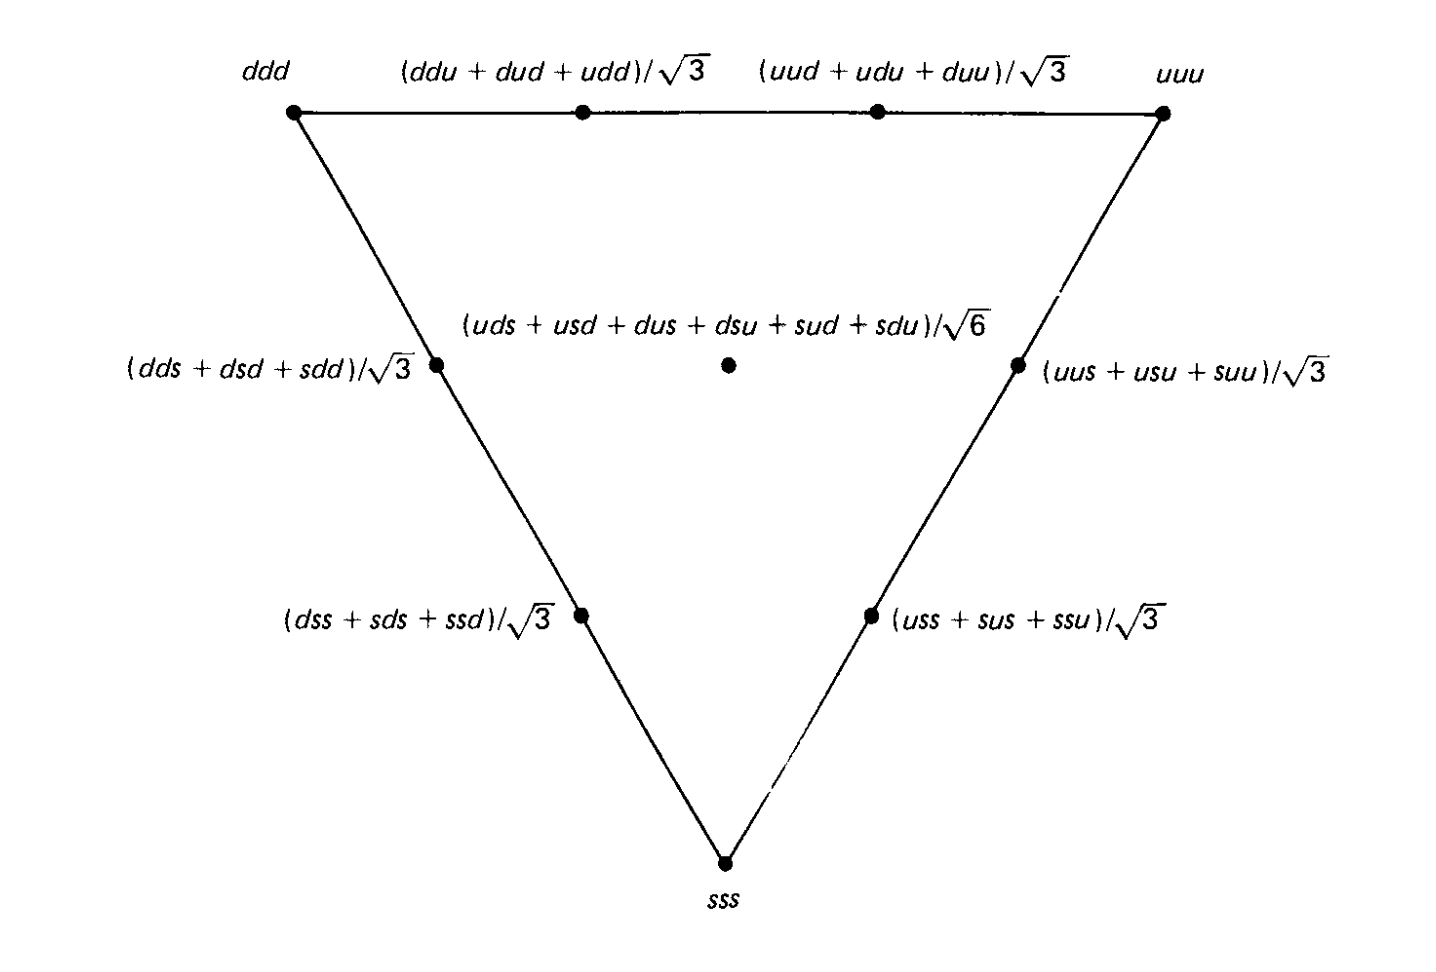
\includegraphics[width=0.5\textwidth]{decuplet.png}
            \caption{Decuplet}
            \label{fig:invertedcolor}
        \end{figure}
        The figure has isospin $I_3$ on the x-axis and spin $S$ on the y-axis.
        We know that the quark charges are
        \begin{align*}
            u = \frac{2}{3} \qquad d = -\frac{1}{3} \qquad s = -\frac{1}{3}
        \end{align*}
        So the top right is (uuu) and etc. for the other corners. But these states are symmetric and
        the spin is also symmetric so we need something else that needs to be antisymmetric. Thus
        we have colors in $SU(3)_c$:
        \begin{align*}
            q = \mqty(r \\ g \\ b)
        \end{align*}
        this also by $SU(3)$ algebra has 27 states of color:
        \begin{align*}
            3 \otimes 3 \otimes 3 = 10 \oplus 8 \oplus 8 \oplus 1
        \end{align*}
        but....
        \begin{quote}
            \textbf{Every Naturally Occuring Particle is a Color Singlet - Griffiths}
        \end{quote}
        AKA the \emph{Color Confinement} principle. So the singlet is always antisymmetric:
        \begin{align*}
            \psi = \frac{1}{\sqrt{6}} (rgb - rbg + gbr - grb + brg - bgr)
        \end{align*}
    \end{itemize}
    So since everything except color is must be symmetric for the total to be antisymmetric i.e.
    \begin{align*}
        \psi(spin) \psi(flavor) = \text{symmetric}
    \end{align*}
    So how do we get from $\Delta^{++}$ to $\Delta^+$? We use the $I_-$ operator:
    From the lowering operator
    \begin{align*}
        J_- \ket{j, m} = \hbar \sqrt{(j + m)(j - m + 1)} \ket{j, m-1}
    \end{align*}
    so in isospin-space
    \begin{align*}
        u = \ket{\ohf, \ohf}
    \end{align*}
    thus
    \begin{align*}
        I_- u = I_- \ket{\ohf, \ohf} = \hbar \sqrt{\ohf(\ohf + 1) - \ohf(\ohf - 1)} \ket{\ohf, -\ohf}
            = \hbar \sqrt{1} \ket{\ohf, -\ohf} = d
    \end{align*}
    and we also get
    \begin{align*}
        I_- d = 0 \qqtext{lowest $I_3$ state} \\
        I_- s = 0 \qqtext{singlet}
    \end{align*}
    SO 
    \begin{align*}
        I_- \Delta^{++} &= I_- (uuu) =  (uud + udu + duu) \\
        I_- \ket{\thf, \thf} &= \sqrt{3} \ket{\thf, \ohf} \\
        &= \sqrt{3} \Delta^+ \\
        \implies \Delta^+ &= \frac{1}{\sqrt{3}} (uud + udu + duu)
    \end{align*}
    applying the lowering operator again we get
    \begin{align*}
        \Delta^0 &= \frac{1}{\sqrt{3}} (udd + dud + ddu) \\
    \end{align*}
    and again
    \begin{align*}
        \Delta^- = ddd
    \end{align*}
    and for the $\Sigma$ (strangeness $S = -1$) states we have the following:
    \begin{align*}
        \Sigma^{*+} &= \frac{1}{\sqrt{3}} (uus + usu + suu) \\
        \Sigma^{*0} &= \frac{1}{\sqrt{3}} (uds + dus + dsu + sud + sdu + uds) \\
        \Sigma^{*-} &= \frac{1}{\sqrt{3}} (dds + dsd + sdd)
    \end{align*}
    for $S = -2$ we have the 2 $\Xi$ states:
    \begin{align*}
        \Xi^{*0} &= \frac{1}{\sqrt{3}} (uss + sus + ssu) \\
        \Xi^{*-} &= \frac{1}{\sqrt{3}} (dss + sds + ssd)
    \end{align*}
    and a singlet 
    \begin{align*}
        \Omega^- = sss
    \end{align*}
    so the flavor is symmetric for the decuplet states
    \paragraph*{Octet States} 
    \begin{figure*}[ht]
        \centering
        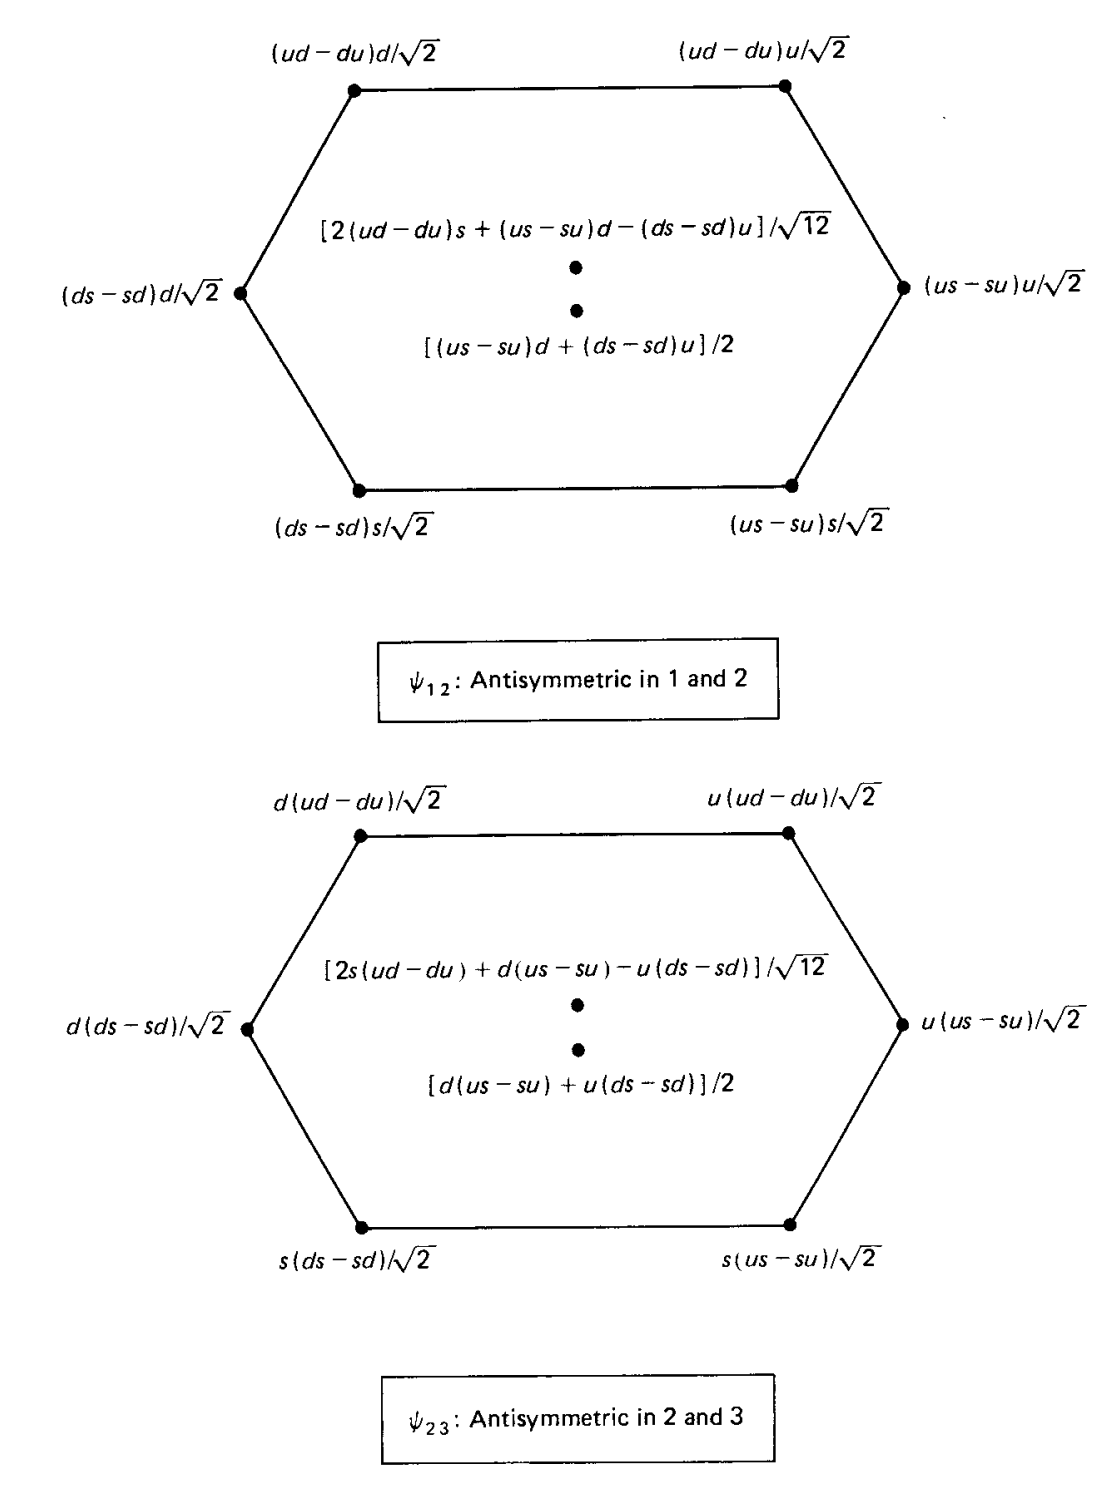
\includegraphics[width=0.5\textwidth]{2octets.png}
        \caption{1st and 2nd Octets}
        \label{fig:octet}
    \end{figure*}
    In the first octet we have 8 states
    \begin{itemize}
        \item n, p 
        \item $\Sigma^+, \Sigma^0, \Sigma^-$
        \item $\Xi^0, \Xi^-$
        \item $\Lambda^0$
    \end{itemize}
    now we need to do the same partial antisymmetry thing we did for spins onto the flavor states:
    \begin{align*}
        \psi(flavor) = \ket{\;}_{12} \qor \ket{\;}_{23} \qor \ket{\;}_{13}
    \end{align*}
    since the proton is a quark made of $uud$ we know that
    \begin{align*}
        \ket{\;}_{12} &= \frac{1}{\sqrt{2}} (ud - du)u \\
        \ket{p(s_z = \ohf)} &= \frac{1}{\sqrt{2}} (ud - du)u \otimes \frac{1}{\sqrt{2}} (\ua\da - \da\ua)\ua \\
        &= \frac{1}{2} [u(\ua) d(\da) u(\ua) \\
        &\qquad - u(\da) d(\ua) u(\ua) \\
        &\qquad - d(\ua) u(\da) u(\ua) \\
        &\qquad + d(\da) u(\ua) u(\ua)] \\
    \end{align*}
    and we can do this for the flavor and spin wavefunctions:
    \begin{align*}
        \psi(flavor) \psi(spin) &= \frac{\sqrt{2}}{3} [\psi_{12}(f)\psi_{12}(s) \\
        &\qquad + \psi_{23}(f)\psi_{23}(s) \\
        &\qquad + \psi_{13}(f)\psi_{13}(s)]
    \end{align*}
where the will have to find this constant in HW. Thus the proton is
\begin{align*}
    \ket{p(\text{spin up})} &= \frac{1}{2 }\sqrt{2}{3} [(ud -du)u (\ua\da - \da\ua)\ua \\
    &\qquad + u(ud - da) \ua(\ua\da - \da\ua) \\
    &\qquad + (uud - duu) (\ua\ua\da - \da\ua\ua)] \\
    &= \frac{1}{3\sqrt{2}} [uud(2\ua\ua\da - \ua\da\ua - \da\ua\ua) \\
    &\qquad + udu(2\ua\da\ua - \da\ua\ua - \ua\ua\da) \\
    &\qquad + duu(-\ua\da\ua + 2\da\ua\ua - \ua\ua\da)]
\end{align*}
so for $n$ we have
\begin{align*}
    \ket{n}_{12} = \frac{1}{\sqrt{2}} (ud -du)d 
\end{align*}
and for sigma
\begin{align*}
    \ket{\Sigma^+}_{12} &= \frac{1}{\sqrt{2}} (us -su)u \\
    \ket{\Xi^0}_{12} &= \frac{1}{\sqrt{2}} (us -su)s
\end{align*}
\end{itemize}

\newpage
\lhead{Lecture 14: 3/4/24}
\paragraph*{Quiz Review (From last time)}
We found for the baryon wavefunction that the space part is symmetric ($\ell = 0$), the spin \&
flavor parts are symmetric, and the color part is antisymmetric. For the spin up proton:
\begin{align*}
    \psi = \frac{\sqrt 2}{3} \qt[\psi_{12}(spin) \psi_{12}(flavor) + \psi_{23}(spin) \psi_{23}(flavor) + \psi_{13}(spin) \psi_{13}(flavor)]
\end{align*}
where
\begin{align*}
    \braket{\psi_{12}}{\psi_{23}} \neq 0 \qquad \braket{\psi_{12}}{\psi_{13}} \neq 0 
\end{align*}
and
\begin{align*}
    \psi_{12}(spin) &= \frac{1}{\sqrt 2} (\ua\da- \da\ua)\ua \\
    \psi_{12}(flavor) &= \frac{1}{\sqrt 2} (ud - du)u
\end{align*}
so the wavefunction of the two parts is
\begin{align*}
    \psi = \frac{\sqrt 2}{3} \qt[2u(\ua) u(\ua) d(\da) - u(\ua) u(\da) d(\ua) - u(\da) u(\ua) d(\ua) 
    + \text{permuations}]
\end{align*}
\paragraph*{Magnetic Moment} The experimental test, the magnetic moment
\begin{align*}
    \vb*\mu = \frac{q}{mc} \vb S
\end{align*}
where the Hamiltonian is
\begin{align*}
    H = -\vb*\mu \cdot \vb B
\end{align*}
and the magnetic moment of a baryon is a vector sum of the three quarks
\begin{align*}
    \vb*\mu(\text{baryon}) = \vb*\mu_1 + \vb*\mu_2 + \vb*\mu_3
\end{align*}
so the $z$-component of the magnetic moment is
\begin{align*}
    \mu_z(\text{baryon}) = \sum_i \mu_{i_z} = \sum_i \frac{q_i}{mc} S_{i_z}
\end{align*}
where
\begin{align*}
    \mu_{i_z} = \frac{q_i}{mc} \frac{\hbar}{2}
\end{align*}
so for each quark
\begin{align*}
    \mu_u = \frac{2}{3} \frac{\hbar}{2m_u c} \qquad \mu_d = -\frac{1}{3} \frac{\hbar}{2m_d c} 
    \qquad \mu_s = -\frac{1}{3} \frac{\hbar}{2m_s c}
\end{align*}
so the expectation value of the magnetic moment operator $\mu_z$ is
\begin{align*}
    \mu_{\text{baryon}, \ua} &= \bra{B(\ua)} \mu_z \ket{B(\ua)} \\
    &= \sum_i \bra{B(\ua)} \mu_{i_z} \ket{B(\ua)} \\
    &= \frac{2}{\hbar} \sum_i \bra{B(\ua)} \mu_i S_{i_z} \ket{B(\ua)}
\end{align*}
So calculating the expectation value for the proton
\begin{align*}
    \sum_i \mu_i S_{i_z} \ket{u(\ua) u(\ua) d(\da)} &=
         \qt(\mu_u \frac{\hbar}{2} + \mu_u \frac{\hbar}{2} + \mu_d \frac{-\hbar}{2}) 
         \ket{u(\ua) u(\ua) d(\da)}
\end{align*}
the first term is 
\begin{align*}
    \mu_1 &= \sum_i \bra{p(\ua)} \mu_i S_{i_z} \ket{p(\ua)} \\
    &= \qt(\frac{2}{3\sqrt 2})^2 \frac{\hbar}{2} (2\mu_u - \mu_d) \frac{2}{\hbar}
        \bra{u(\ua) u(\ua) d(\da)} \ket{u(\ua) u(\ua) d(\da)} \\
    &= \frac{2}{9} (2\mu_u - \mu_d)
\end{align*}
the second term $-u(\ua) u(\da) d(\ua)$ is
\begin{align*}
    \frac{\hbar}{2} (\mu_u - \mu_u + \mu_d) = \frac{\hbar}{2} \mu_d
\end{align*}
so
\begin{align*}
    \qt(\frac{1}{3\sqrt 2})^2 \mu_d = \frac{1}{18} \mu_d
\end{align*}
and same for the third term. We get the magnetic moment as
\begin{align*}
    \mu_{p(\ua)} &= 3 \qt[\frac{2}{9} (2\mu_u - \mu_d) + \frac{1}{18} \mu_d + \frac{1}{18} \mu_d] \\
    &= \frac{3}{18} (4(2\mu_u - \mu_d) + 2\mu_d) \\
    &= \frac{1}{6} (8\mu_u - 2\mu_d ) \\
    &= \frac{1}{3} (4\mu_u - \mu_d)
\end{align*}
and from the experimental values:
\begin{align*}
    m_p = 2.79 m_u = 2.79 m_d
\end{align*}
we get
\begin{align*}
    \mu_p = 2.79 \frac{e\hbar}{2m_p c} = 2.79 \mu_B
\end{align*}
where $\mu_B = \frac{e\hbar}{2m_p c}$ is the Bohr magneton. And for the neutron we know
\begin{align*}
    p: uud \qquad n: udd
\end{align*}
so all we have to do is replace the $u$ with $d$ and thus:
\begin{align*}
    \mu_n &= \frac{1}{3} (4\mu_d - \mu_u) \\
    &= \frac{1}{3} \qt(4(-1/3) \frac{\hbar}{2m_d c} - 2/3 \frac{\hbar}{2m_u c}) \\
    &= -\frac{2}{3} (2.79) \frac{e\hbar}{2m_p c} = -1.86 \mu_B
\end{align*}
experimentally, we got the proton and neutron magnetic moments to be
\begin{align*}
    \mu_p &= 2.793 \mu_B \qquad \mu_n = -1.913 \mu_B
\end{align*}
we can also take the ratio of the magnetic moments
\begin{align*}
    \frac{\mu_n}{\mu_p} = -\frac{2}{3}
\end{align*}
which is independent of the quark masses! This is a (robust) prediction of the quark model

\paragraph*{If there was no color} Then the wavefunction would be
\begin{align*}
    \psi = \psi_{space} \psi_{spin} \psi_{flavor}
\end{align*}
so
\begin{align*}
    \psi(spin) \psi(flavor) = \text{anti-symmetric}
\end{align*}
and we would get the ratio of the magnetic moments to be
\begin{align*}
    \frac{\mu_n}{\mu_p} = -2
\end{align*}

\paragraph*{Baryon Masses} For the meson masses we had the mass as the sum of the masses and the
spin-spin interaction:
\begin{align*}
    M = m_1 + m_2 + A \frac{\vb S_1 \cdot \vb S_2}{m_1 m_2}
\end{align*}
But for the baryons we have 3 quarks so we have
\begin{align*}
    M = m_1 + m_2 + m_3 + A' \qt(\frac{\vb S_1 \cdot \vb S_2}{m_1 m_2} 
        + \frac{\vb S_1 \cdot \vb S_3}{m_1 m_3} 
        + \frac{\vb S_2 \cdot \vb S_3}{m_2 m_3})
\end{align*}
For the decuplet we have the inverted triangle from Figure \ref{fig:invertedcolor} and the octet 
from Figure \ref{fig:octet}. Taking $m_u = m_d$
\begin{itemize}
    \item For Baryons with no $S$,
    \begin{align*}
        M &= 3\mu_u + \frac{A'}{m_\mu^2}(\vb S_1 \cdot \vb S_2 + \vb S_1 \cdot \vb S_3 + \vb S_2 \cdot \vb S_3)
    \end{align*}
    so the total spin is
    \begin{align*}
        \vb S^2 &= (\vb S_1 + \vb S_2 + \vb S_3)^2 \\
        &= \vb S_1^2 + \vb S_2^2 + \vb S_3^2 + 2(\vb S_1 \cdot \vb S_2 + \vb S_1 \cdot \vb S_3 + \vb S_2 \cdot \vb S_3) \\
        \implies & \vb S_1 \cdot \vb S_2 + \vb S_1 \cdot \vb S_3 + \vb S_2 \cdot \vb S_3 = \frac{1}{2} (\vb S^2 - \vb S_1^2 - \vb S_2^2 - \vb S_3^2) = S'
    \end{align*}
    where the eigen values are
    \begin{align*}
        \ohf (\ohf + 1) \hbar^2 = \frac{3}{4} \hbar^2
    \end{align*}
    i.e.
    \begin{align*}
        s = 3/2: \vb S^2 = \frac{3}{2} (\frac{3}{2} + 1) \hbar^2 = \frac{15}{4} \hbar^2 \\
        s = 1/2: \vb S^2 = \frac{1}{2} (\frac{1}{2} + 1) \hbar^2 = \frac{3}{4} \hbar^2
    \end{align*}
    so
    \begin{align*}
        &= \ohf \qt(\vb S^2 - 3 \frac{3}{4} \hbar^2) \\
        &= \ohf \begin{cases}
            \frac{3}{2} \hbar^2 & S = \frac{3}{2} \qqtext{(decuplet)} \\
            -\frac{3}{2} \hbar^2 & S = \frac{1}{2} \qqtext{(octet)}
        \end{cases}
    \end{align*}
    so the masses are
    \begin{align*}
        M_N = 3m_u - \frac{3}{4} \frac{\hbar^2}{m_u^2} A' \\
        M_\Delta = 3m_u + \frac{3}{4} \frac{\hbar^2}{m_u^2} A'
        M_\Omega = 3m_s + \frac{3}{4} \frac{\hbar^2}{m_s^2} A'
    \end{align*}
    For the decuplet case all spin are parallel so for $s = 3/2$:
    \begin{align*}
        \vb S_1 \cdot \vb S_2 = \vb S_1 \cdot \vb S_3 = \vb S_2 \cdot \vb S_3 = \frac{1}{4} \hbar^2
    \end{align*}
    and
    \begin{align*}
        (\vb S_1 + \vb S_2)^2 &= \vb S_1^2 + \vb S_2^2 + 2\vb S_1 \cdot \vb S_2 \\
        \vb S_1 \cdot \vb S_2 &= \frac{1}{2} (\vb S^2 - \vb S_1^2 - \vb S_2^2) = \frac{3}{4} \hbar^2
        &= \frac{1}{2} \qt(1(1 + 1)\hbar^2 - 2 \frac{3}{4}\hbar^2) = \frac{1}{4} \hbar^2
    \end{align*}
    so the maasses are calculated  by:
    \begin{align*}
        M = m_1 + m_2 + m_3 + \frac{A'}{4}\hbar^2 \qt(\frac{1}{m_1 m_3} + \frac{1}{m_2 m_3} + \frac{1}{m_2 m_3})
    \end{align*}
    For the octet case
    \begin{align*}
        M_\Sigma: (ud) \quad I = 1 \\
        M_\Lambda: (ud) \quad I = 0 \\
    \end{align*}
    so for example the $\Sigma^+$ case:
    \begin{align*}
        M_{\Sigma^+} &= 2m_u + m_s + A' \qt(\frac{\vb S_u \cdot \vb S_u}{m_u^2} 
            + \frac{\vb S_u \cdot \vb S_s}{m_u m_s} + \frac{\vb S_u \cdot \vb S_s}{m_u m_s})
    \end{align*}
    and since we have already calculated 
    \begin{align*}
        \vb S_u \cdot \vb S_u = \frac{1}{4} \hbar^2 
    \end{align*}
    and we know the spin for the octet is
    \begin{align*}
        \vb S_u \cdot \vb S_u + \vb S_{u1} \cdot \vb S_s + \vb S_{u2} \cdot \vb S_s = -\frac{3}{4} \hbar^2
        \vb S_{u1} \cdot \vb S_s + \vb S_{u2} \cdot \vb S_s = - \hbar^2
    \end{align*}
    and from anti symmetry we know that
    \begin{align*}
        \vb S_{u1} = \vb S_{u2} = -\frac{3}{2} \hbar^2
    \end{align*}
    and we can do the same for the other octet states.
\end{itemize}
Midterm: Multiple choice 25pt, bound states(general structure why $1/n^2$) heavy masses, wavefunctions,
relativistic kinematics. 
\end{document}